\documentclass{article}

% packages
\usepackage{amsmath, amsthm, thmtools, amsfonts, amssymb, luacode, catchfile, tikzducks, hyperref, ifthen}
\ifcsname c@kobocompile\endcsname
	\usepackage[a5paper, total={1072pt, 1448pt}, margin=10pt, includeheadfoot]{geometry} % set page margins
\else
	\usepackage[a4paper, margin=50pt, includeheadfoot]{geometry}
\fi
\usepackage[shortlabels]{enumitem}
\usepackage[skip=3pt, indent=0pt]{parskip}

% language
\usepackage[bidi=basic, layout=tabular, provide=*]{babel}
\ifcsname c@english\endcsname
	\babelprovide[main, import]{english}
\else
	\babelprovide[main, import]{hebrew}
	\babelprovide{rl}
\fi
%\babelfont{rm}{Libertinus Serif}
\babelfont{rm}[Renderer=Harfbuzz]{Libertinus Serif}
\babelfont{sf}{Libertinus Sans}
\babelfont{tt}{Libertinus Mono}

% style
\AddToHook{cmd/section/before}{\clearpage}	% Add line break before section
\linespread{1.3}
\setcounter{secnumdepth}{0}		% Remove default number tags from sections, this won't do well with theorems
\AtBeginDocument{\setlength{\belowdisplayskip}{3pt}}
\AtBeginDocument{\setlength{\abovedisplayskip}{3pt}}
\graphicspath{ {../images/} }

% operators
\DeclareMathOperator\cis{cis}
\DeclareMathOperator\Sp{Sp}
\DeclareMathOperator\tr{tr}
\DeclareMathOperator\im{Im}
\DeclareMathOperator\re{Re}
\DeclareMathOperator\diag{diag}
\DeclareMathOperator*\lowlim{\underline{lim}}
\DeclareMathOperator*\uplim{\overline{lim}}
\DeclareMathOperator\rng{rng}
\DeclareMathOperator\Sym{Sym}
\DeclareMathOperator\Arg{Arg}
\DeclareMathOperator\Log{Log}
\DeclareMathOperator\dom{dom}
\DeclareMathOperator\supp{Supp}
\DeclareMathOperator\var{Var}
\DeclareMathOperator\cov{Cov}

% commands
%\renewcommand\qedsymbol{\textbf{מש''ל}}
%\renewcommand\qedsymbol{\fbox{\emoji{lizard}}}
\newcommand{\Aa}[0]{\mathcal{A}}
\newcommand{\Bb}[0]{\mathcal{B}}
\newcommand{\CC}[0]{\mathbb{C}}
\newcommand{\Cc}[0]{\mathcal{C}}
\newcommand{\EE}[0]{\mathbb{E}}
\newcommand{\FF}[0]{\mathbb{F}}
\newcommand{\Ff}[0]{\mathcal{F}}
\newcommand{\Ii}[0]{\mathcal{I}}
\newcommand{\Gg}[0]{\mathcal{G}}
\newcommand{\Ll}[0]{\mathcal{L}}
\newcommand{\Mm}[0]{\mathcal{M}}
\newcommand{\NN}[0]{\mathbb{N}}
\newcommand{\Nn}[0]{\mathcal{N}}
\newcommand{\PP}[0]{\mathbb{P}}
\newcommand{\Pp}[0]{\mathcal{P}}
\newcommand{\QQ}[0]{\mathbb{Q}}
\newcommand{\RR}[0]{\mathbb{R}}
\newcommand{\Rr}[0]{\mathcal{R}}
\newcommand{\Ss}[0]{\mathcal{S}}
\newcommand{\TT}[0]{\mathbb{T}}
\newcommand{\Uu}[0]{\mathcal{U}}
\newcommand{\Vv}[0]{\mathcal{V}}
\newcommand{\Ww}[0]{\mathcal{W}}
\newcommand{\ZZ}[0]{\mathbb{Z}}
\newcommand{\acts}[0]{\circlearrowright}
\newcommand{\explain}[2] {
	\begin{flalign*}
		 && \text{#2} && \text{#1}
	\end{flalign*}
}
\newcommand{\maketitleprint}[0]{ \begin{center}
	%\begin{tikzpicture}[scale=3]
	%	\duck[graduate=gray!20!black, tassel=red!70!black]
	%\end{tikzpicture}	
	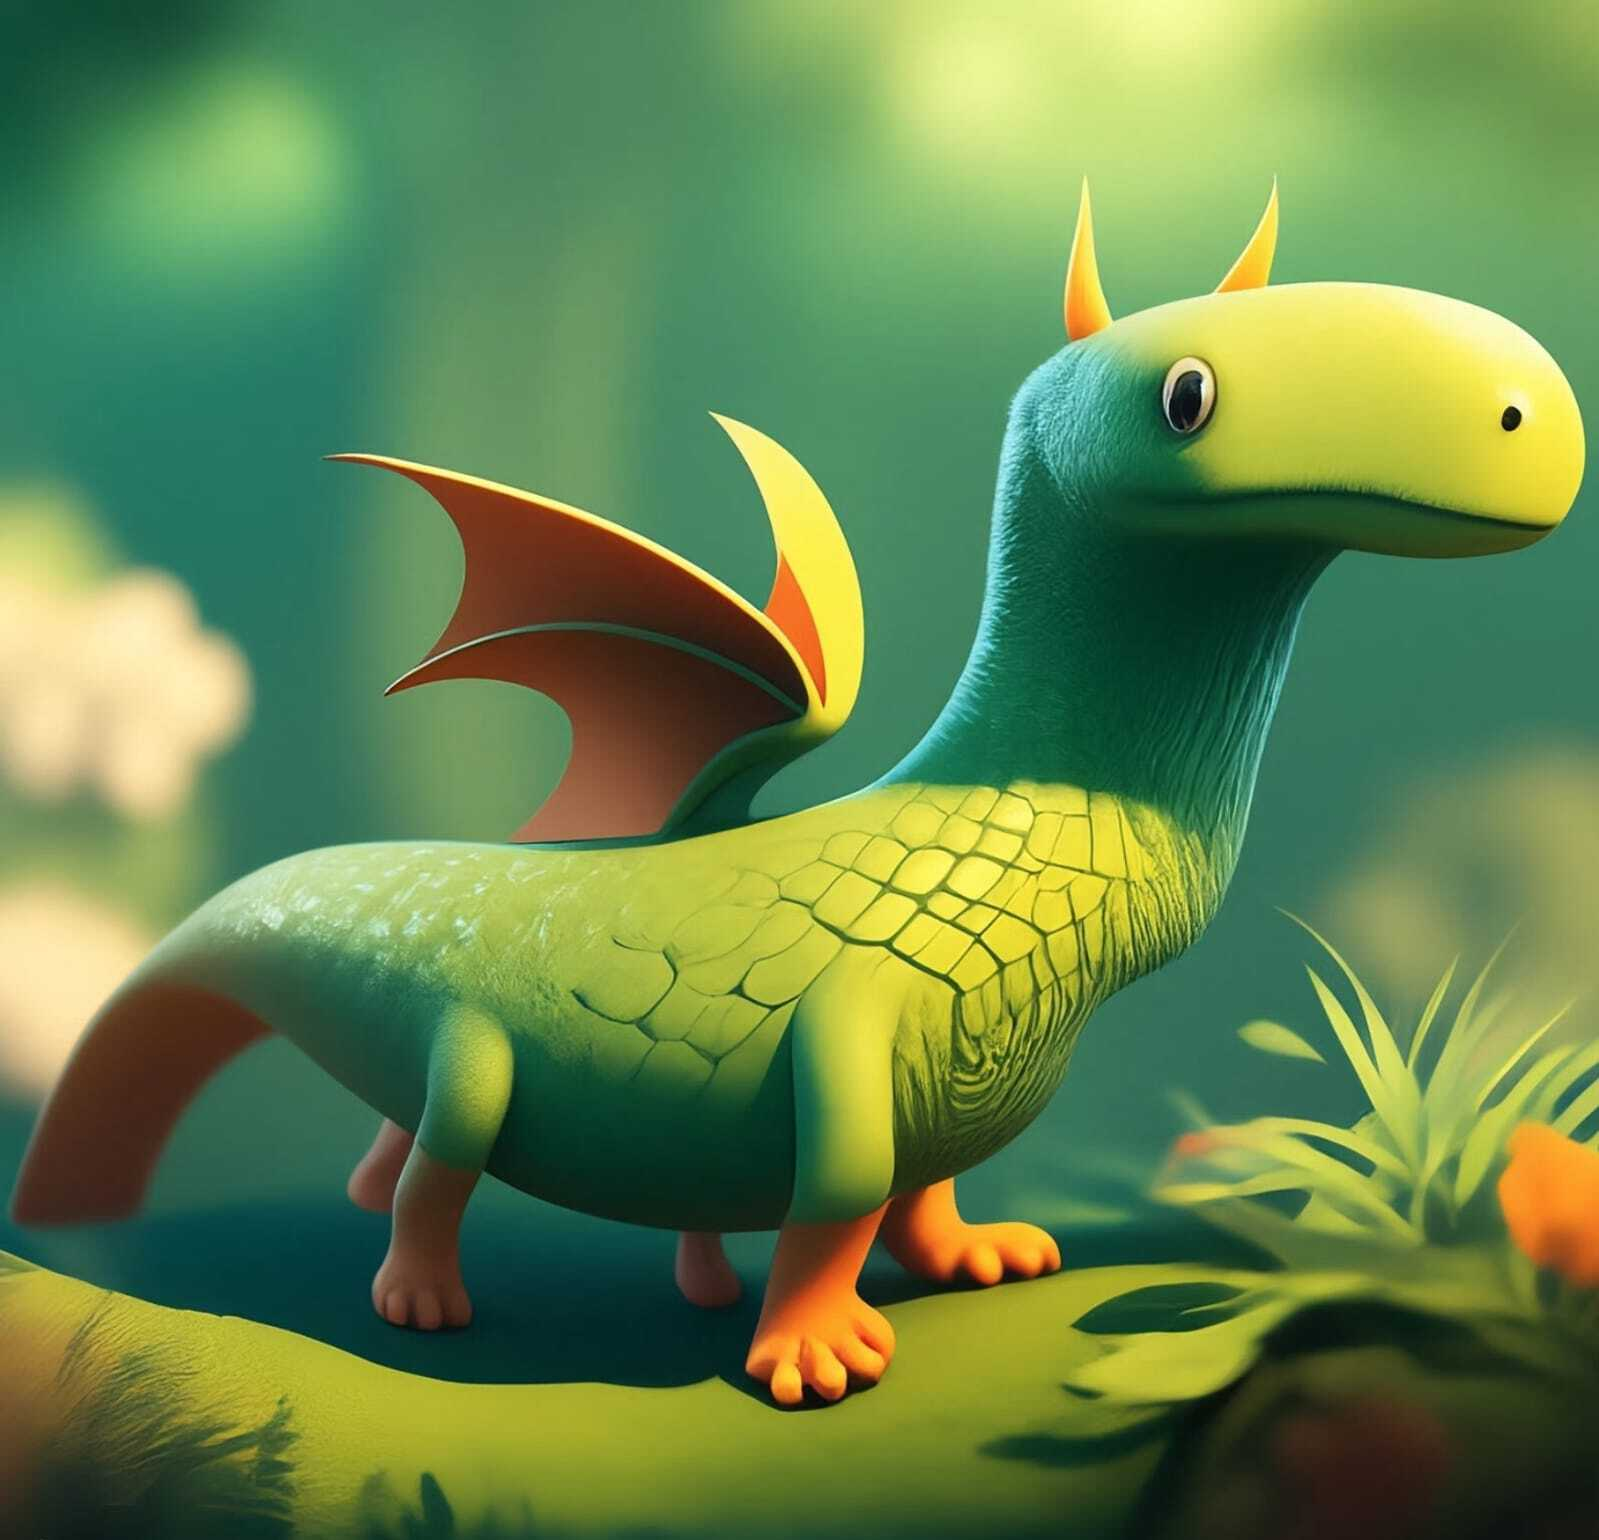
\includegraphics[width=6cm]{cover}
\end{center}
}

% theorem commands
\newtheoremstyle{c_remark}
	{}	% Space above
	{}	% Space below
	{}% Body font
	{}	% Indent amount
	{\bfseries}	% Theorem head font
	{}	% Punctuation after theorem head
	{.5em}	% Space after theorem head
	{\thmname{#1}\thmnumber{ #2}\thmnote{ \normalfont{\text{(#3)}}}}	% head content
\newtheoremstyle{c_definition}
	{3pt}	% Space above
	{3pt}	% Space below
	{}% Body font
	{}	% Indent amount
	{\bfseries}	% Theorem head font
	{}	% Punctuation after theorem head
	{.5em}	% Space after theorem head
	{\thmname{#1}\thmnumber{ #2}\thmnote{ \normalfont{\text{(#3)}}}}	% head content
\newtheoremstyle{c_plain}
	{3pt}	% Space above
	{3pt}	% Space below
	{\itshape}% Body font
	{}	% Indent amount
	{\bfseries}	% Theorem head font
	{}	% Punctuation after theorem head
	{.5em}	% Space after theorem head
	{\thmname{#1}\thmnumber{ #2}\thmnote{ \text{(#3)}}}	% head content

\ifcsname c@english\endcsname
	\theoremstyle{plain}
	\newtheorem{theorem}{Theorem}[section]
	\newtheorem{lemma}[theorem]{Lemma}
	\newtheorem{proposition}[theorem]{Proposition}
	\newtheorem*{proposition*}{Proposition}
	%\newtheorem{corollary}[theorem]{אין חלופה עברית}

	\theoremstyle{definition}
	\newtheorem{definition}[theorem]{Definition}
	\newtheorem*{definition*}{Definition}
	\newtheorem{example}{Example}[section]
	\newtheorem{exercise}{Exercise}[section]

	\theoremstyle{remark}
	\newtheorem*{remark}{Remark}
	\newtheorem*{solution}{Solution}
	\newtheorem{conclusion}[theorem]{Conclusion}
	\newtheorem{notation}[theorem]{Notation}
\else
	\theoremstyle{c_plain}
	\newtheorem{theorem}{משפט}[section]
	\newtheorem{lemma}[theorem]{למה}
	\newtheorem{proposition}[theorem]{טענה}
	\newtheorem*{proposition*}{טענה}
	%\newtheorem{corollary}[theorem]{אין חלופה עברית}

	\theoremstyle{c_definition}
	\newtheorem{definition}[theorem]{הגדרה}
	\newtheorem*{definition*}{הגדרה}
	\newtheorem{example}{דוגמה}[section]
	\newtheorem{exercise}{תרגיל}[section]

	\theoremstyle{c_remark}
	\newtheorem*{remark}{הערה}
	\newtheorem*{solution}{פתרון}
	\newtheorem{conclusion}[theorem]{מסקנה}
	\newtheorem{notation}[theorem]{סימון}
\fi

% Questions related commands
\newcounter{question}
\setcounter{question}{1}
\newcounter{sub_question}
\setcounter{sub_question}{1}

\ifcsname c@english\endcsname
	\newcommand{\question}[1][0]{
		\ifthenelse{#1 = 0}{}{\setcounter{question}{#1}}
		\section{Question \arabic{question}}
		\addtocounter{question}{1}
		\setcounter{sub_question}{1}
	}

	\newcommand{\subquestion}[1][0]{
		\ifthenelse{#1 = 0}{}{\setcounter{sub_question}{#1}}
		\subsection{Part \alph{sub_question}}
		\addtocounter{sub_question}{1}
	}
\else
	\newcommand{\question}[1][0]{
		\ifthenelse{#1 = 0}{}{\setcounter{question}{#1}}
		\section{שאלה \arabic{question}}
		\addtocounter{question}{1}
		\setcounter{sub_question}{1}
	}

	\newcommand{\subquestion}[1][0]{
		\ifthenelse{#1 = 0}{}{\setcounter{sub_question}{#1}}
		\subsection{סעיף \localecounter{letters.gershayim}{sub_question}}
		\addtocounter{sub_question}{1}
	}
\fi

% import lua and start of document
\directlua{common = require ('../common')}

\GetEnv{AUTHOR}

% headers
\author{\AUTHOR}
\date\today

\title{מבוא לטופולוגיה --- סיכום}
\setcounter{secnumdepth}{2}
% chktex-file 9
% chktex-file 17

\usepackage{fancyhdr}
\pagestyle{fancy}
\renewcommand{\headrulewidth}{0pt}

\begin{document}
\maketitle
\maketitleprint{}

\tableofcontents

\section{שיעור 1 --- 24.3.2025}
\subsection{מבוא}
בעבר דיברנו על מרחבים מטריים, באינפי 1 מתבוננים ב־$\RR$ והגדרנו את מושג הגבול של סדרות, ולאחריו את המושג של פונקציה רציפה $f : \RR \to \RR$.
ההגדרה הייתה ש־$f$ תיקרא רציפה אם לכל $x \in \RR$ ולכל $\lim_{n \to \infty} x_n = x$ מתקיים $\lim_{n \to \infty} f(x_n) = f(x)$.
באינפי 3 כבר ראינו את המושג הכללי והרחב יותר של רציפות במרחבים מטריים.
ניזכר בהגדרה של מרחב מטרי.
\begin{definition}[מרחב מטרי]
	מרחב מטרי הוא זוג $(X, d)$ כאשר $X$ קבוצה לא ריקה ו־$d : X \times X \to \RR$ פונקציה (הנקראת מטריקה) המקיימת,
	\begin{enumerate}
		\item $d(x, y) = d(y, x)$ לכל $x, y \in X$
		\item $\forall x, y \in X, d(x, y) \ge 0$ וכן $d(x, y) = 0 \iff x = y$
		\item אי־שוויון המשולש, $\forall x, y, z \in X, d(x, y) \le d(x, y) + d(y, z)$
	\end{enumerate}
\end{definition}
\begin{example}
	נראה דוגמות למרחבים מטריים,
	\begin{enumerate}
		\item $\RR$ יחד עם $d(x, y) = |x - y|$
		\item $(\RR^n, d_2)$ המוגדרת על־ידי $d_2(\bar{x}, \bar{y}) = \sqrt{\sum_{i = 1}^{n} {|x_i - y_i|}^2}$
		\item נוכל עבור $\RR^n$ להגדיר את $d_p(\bar{x}, \bar{y}) = {(\sum_{i = 1}^{n} {|x_i - y_i|}^p)}^\frac{1}{p}$ ואת מטריקת אינסוף, $d_\infty(\bar{x}, \bar{y}) = \max_{1 \le i \le n} |x_i - y_i|$
		\item עבור $C([a, b])$ קבוצת הפונקציות הרציפות $[a, b] \to \RR$ עבור $a < b$, ונגדיר את המטריקה $\rho(f, g) = \sup_{x \in [a, b]} |f(x) - g(x)|$
	\end{enumerate}
\end{example}
נראה את ההגדרה הפורמלית של רציפות,
\begin{definition}[רציפות]
	תהי $f : X \to Y$ עבור $(X, d), (Y, \rho)$ מרחבים מטריים, אז נאמר ש־$f$ רציפה אם ורק אם לכל $\epsilon > 0$ קיים $\delta > 0$ כך שאם $d(x', x) < \delta$ אז $\rho(f(x'), f(x)) < \epsilon$.
\end{definition}
אבל יותר קל לדבר במונחים של קבוצות פתוחות.
\begin{definition}[כדור]
	עבור $(X, d)$ מרחב מטרי,
	נסמן $B(r, x) = B_r(x) = \{ z \in X \mid d(x, z) < r \}$.
\end{definition}
\begin{definition}[קבוצה פתוחה]
	יהי $(X, d)$ מרחב מטרי, תת־קבוצה $U \subseteq X$ תיקרא פתוחה אם לכל $x \in U$ קיים $r > 0$ כך ש־$x \in B(x, r) \subseteq U$.
\end{definition}
\begin{definition}[הגדרה שקולה לרציפות]
	$f : X \to Y$ תיקרא רציפה אם לכל $V \subseteq Y$ קבוצה פתוחה ב־$Y$ מתקיים $f^{-1}(V) = \{ x \in X \mid f(x) \in V \}$ קבוצה פתוחה ב־$X$.
\end{definition}
\begin{definition}[טופולוגיה]
	תהי $X$ קבוצה (לא ריקה), \textbf{טופולוגיה} על $X$ היא אוסף $\tau \subseteq \Pp(X)$, כך שמתקיימים התנאים הבאים,
	\begin{enumerate}
		\item $X, \emptyset \in \tau$
		\item $\tau$ סגור לאיחוד, כלומר אם ${\{U_\alpha\}}_{\alpha \in I}$ לקבוצת אינדקסים $I$, כך ש־$\forall \alpha \in I, U_\alpha \in \tau$ אז $\bigcup_{\alpha \in I} U_\alpha \in \tau$
		\item $\tau$ סגור לחיתוכים סופיים, כלומר לכל $U, V \in \tau$ מתקיים $U \cap V \in \tau$
	\end{enumerate}
\end{definition}
\begin{definition}[מרחב טופולוגי]
	זוג $(X, \tau)$ כאשר $X$ קבוצה לא ריקה ו־$\tau$ טופולוגיה על $X$, יקרא מרחב טופולוגי.
\end{definition}
\begin{remark}
	בעצם הגדרנו כבר מתי פונקציה $f : X \to Y$ עבור מרחבים טופולוגיים $(X, \tau), (Y, \Omega)$ היא רציפה, כאשר $f^{-1}(U) \in \tau$ לכל $U \in \Omega$.
\end{remark}
\begin{notation}
	איברי $\tau$ יקראו קבוצות פתוחות.
\end{notation}
\begin{definition}
	אם $(X, \tau)$ מרחב טופולוגי אז תת־קבוצה $A \subseteq X$ תיקרא סגורה אם $X \setminus A \in \tau$, כלומר המשלים של $A$ היא קבוצה פתוחה.
\end{definition}
\begin{example}
	יהי $(X, d)$ מרחב מטרי, נגדיר $\tau = \{ U \subseteq X \mid \forall x \in U \exists r > 0, B(x, r) \subseteq U \}$, כלומר נגדיר טופולוגיה באופן טריוויאלי כנביעה מהמרחב המטרי.
\end{example}
\begin{exercise}
	הוכיחו כי אכן זהו מרחב טופולוגי.
\end{exercise}
\begin{example}
	יהי $X$ קבוצה כלשהי, אז ניתן להגדיר על $X$ טופולוגיה $\tau_0 = \{ \emptyset, X \}$.
	טופולוגיה זו נקראת טופולוגיה טריוויאלית.
\end{example}
\begin{example}
	נגדיר $\tau_1 = \Pp(X)$ עבור קבוצה $X$, גם קבוצה זו היא טופולוגיה, והיא נקראת הטופולוגיה הדיסקרטית.
\end{example}
\begin{example}
	נניח ש־$(Y, \tau)$ מרחב טופולוגי, ותהי $f : (Y, \tau) \to (X, \tau_0)$, מתי $f$ היא רציפה? התשובה היא שהיא רציפה תמיד.
	מתי $f : (Y, \tau) \to (X, \tau_1)$ רציפה? תלוי בהגדרת הפונקציה, אבל במקרה שבו היא אכן רציפה, אז היא רציפה בכל טופולוגיה שהיא.
	לעומת זאת כל $f : (X, \tau_1) \to (Y, \tau)$ היא רציפה.
\end{example}
\begin{remark}
	לא כל טופולוגיה נובעת ממטריקה.
	לדוגמה הטופולוגיה הטריוויאלית על מרחב עם לפחות 2 נקודות.
\end{remark}
\begin{remark}
	נניח $x, y \in X$ אז נבחר $r = \frac{1}{2} d(x, y)$ ואז $y \notin B(x, r)$ ולכן $\emptyset \ne B(x, r) \ne X$, קל לראות שביחס לטופולוגיה שמושרית מהמטריקה $d$, הקבוצה $B(x, r)$ קבוצה פתוחה.
\end{remark}
\begin{example}
	נגדיר $X = \CC^n$ עבור איזשהו $n \in \NN$ ונגדיר $\Ff = \{ A \subseteq \CC^n \mid \exists {\{f_i\}}_{i \in I} \subseteq \CC[x_1, \dots, x_n], A = \{(p_1, \dots, p_n) \mid \forall i \in I, f_i(p_1, \dots, p_n) = 0 \}\}$.
\end{example}
\begin{definition}[בסיס לטופולוגיה]
	בסיס לטופולוגיה הוא אוסף $\Bb$ של תתי־קבוצות של $X$ כך שמתקיים,
	\begin{enumerate}
		\item לכל $x \in X$ יש $B \in \Bb$ כך ש־$x \in B$
		\item לכל $A, B \in \Bb$ ולכל $x \in A \cap B$ יש $C \in \Bb$ כך ש־$x \in C \subseteq A \cap B$
	\end{enumerate}
\end{definition}
\begin{proposition}
	עבור בסיס $\Bb$ האוסף $\tau_\Bb = \{ U \subseteq X \mid U \text{ is a union of elements of } \Bb \}$ היא טופולוגיה,
	\[
		\forall \alpha \in I, B_\alpha \in \Bb, U = \bigcup_{\alpha \in I} B_\alpha
	\]
\end{proposition}
\begin{proof}
	מכיוון ש־$\tau_\Bb$ סגורה לחיתוך סופי, אז אם $U, V \in \tau_\Bb$ אז $U = \bigcup_{\alpha \in I} B_\alpha \in \Bb$ וכן $V = \bigcup_{\beta \in J} A_\beta, A_\beta \in \Bb$, אז מתקיים,
	\[
		U \cap V
		= (\bigcup_{\alpha \in I} B_\alpha) \cap (\bigcup_{\beta \in J} A_\beta)
		= \bigcup_{\alpha, \beta \in I \times J} B_\alpha \cap A_\beta
		= D
	\]
	לכן לכל $x \in U \cap V$ ישנם $\alpha_0 \in I, \beta_0 \in J$ כך ש־$x \in B_{\alpha_0} \cap A_{\beta_0}$,
	אבל מהגדרת הבסיס קיימת קבוצה $C_{\alpha_0, \beta_0} \in \Bb$ כך ש־$C_{\alpha_0, \beta_0} \subseteq B_{\alpha_0} \cap A_{\beta_0}$.
	לכן $D \subseteq \bigcup_{(x, \alpha, \beta)} C_{x, \alpha, \beta}$.
	בהתאם מצאנו סגירות לחיתוך סופי.
\end{proof}
\begin{remark}
	יהי $(X, d)$ מרחב מטרי, אז $\{ B(x, r) \subseteq X \mid x \in X, r > 0 \}$ הוא טופולוגיה.
	אבל עכשיו נוכל להגדיר גם את $\{ B(x, \frac{1}{n}) \subseteq X \mid x \in X, n \in \NN \}$, זהו בסיס לטופולוגיה לאותה הטופולוגיה שהגדרנו למרחב המטרי.
\end{remark}
\begin{exercise}
	הוכיחו שזהו אכן בסיס עבור המרחב הטופולוגי הנתון.
\end{exercise}
\begin{example}
	נניח ש־$X = \ZZ$, ונגדיר את הבסיס $C$ להיות אוסף הסדרות האריתמטיות הדו־צדדיות, כלומר $C = \{ a + d \ZZ \mid a, d \in \ZZ, d \ne 0 \}$.
	אנו טוענים כי זהו אכן בסיס (לטופולוגיה).
	נתבונן בזוג קבוצות ב־$C$, $a + d \ZZ, b + q \ZZ$, ונניח ש־$p \in (a + d \ZZ) \cap (b + q \ZZ)$ אז $p \in p + dq \ZZ \subseteq (a + d \ZZ) \cap (b + q \ZZ)$.
	נגדיר טופולוגיית $\tau_C$.

	קבוצות סגורות הן משלימים לקבוצות פתוחות.

	כל סדרה אריתמטית דו־צדדית אינסופית היא גם פתוחה וגם סגורה.
	בפרט חיתוך סופי של סדרות אריתמטיות הוא סגור.
	לכן המשלים שלו הוא פתוח.
\end{example}
\begin{conclusion}[משפט אוקלידס]
	יש אינסוף מספרים ראשוניים.
\end{conclusion}
\begin{proof}
	נניח בשלילה כי יש מספר סופי של ראשוניים, $p_1, \dots, p_k$ עבור $k \in \NN$.
	נבחן את $\bigcup_{i = 1}^k p_i \ZZ$, זוהי קבוצה פתוחה וגם סגורה, לכן
	\[
		\bigcup_{i = 1}^k p_i \ZZ
		= \ZZ \setminus \{ -1, 1 \}
	\]
	ולכן נובע ש־$\{-1, 1\}$ קבוצה פתוחה וזו כמובן סתירה.
\end{proof}
\begin{proposition}[צמצום מרחב טופולוגי]
	נניח ש־$(X, \tau)$ מרחב טופולוגי, לכל $\emptyset \ne Y \subseteq X$ נגדיר $\tau_Y = \{ U \cap Y \mid U \in \tau \}$.
	אז $\tau_Y$ היא טופולוגיה.
	אם $Y \in \tau$ אז $\tau_Y = \{ W \in \tau \mid W \subseteq Y \}$.
\end{proposition}
\begin{proposition}[טופולוגיית מכפלה]
	נניח ש־$(X_1, \tau_1)$ ו־$(X_2, \tau_2)$ מרחבים טופולוגיים, אז נגדיר טופולוגיה על מרחב המכפלה $X_1 \times X_2$ על־ידי
	\[
		\tau_{1, 2}
		= \{ U_1 \times U_2 \mid U_1 \in \tau_1, U_2 \in \tau_2 \}
	\]
	אז $\tau_{1, 2}$ הוא בסיס והטופולוגיה המוגדרת על־ידו נקראת טופולוגיית המכפלה.
\end{proposition}
\begin{example}
	נוכל לבנות כך מכפלה של כמות סופית או אינסופית של מכפלות טופולוגיות.
	עבור אוסף אינסופי (בן־מניה או לא בהכרח) אנו צריכים להיזהר, נניח ש־$(X_\alpha, \tau_\alpha)$ עבור $\alpha \in I$, אז נגדיר
	\[
		\tau_b = \{ \prod_{\alpha \in I} U_\alpha \mid \forall \alpha \in I, U_\alpha \in \tau_\alpha \}
	\]
	זהו בסיס לטופולוגיה שנקרא טופולוגיית הקופסה.
	לעומת זאת נוכל להגדיר גם את
	\[
		\tau_p
		= \{ \prod_{\alpha \in I} U_\alpha \mid U_\alpha = X_\alpha \text{ for almost all } \alpha \in I \}
	\]
	כלומר $\prod_{\alpha \in I} = \{ f : I \to \bigcup_{\alpha \in I} X_\alpha \mid \forall \alpha \in I, f(x) \in X_\alpha \}$.
\end{example}

\listoftheorems[title=הגדרות ומשפטים,ignoreall,show={theorem,definition},swapnumber,onlynamed={proposition}]

\end{document}
